\documentclass{article}

\usepackage[utf8]{inputenc}
\usepackage[ngerman]{babel}
\usepackage{amssymb}
\usepackage{amsmath}
\usepackage{graphics}
% Pseudocode
\usepackage{algorithm}
\usepackage[noend]{algpseudocode}
\usepackage{graphicx}
\usepackage{pdfpages}

\usepackage{tikz}

\setlength{\parindent}{0in}

\newcommand{\zettelNummer}{9}
\newcommand{\studierenderEins}{Eli Kogan-Wang (7251030)}
\newcommand{\studierenderZwei}{David Noah Stamm (7249709)}
\newcommand{\studierenderDrei}{Daniel Heins (7213874)}
\newcommand{\studierenderVier}{Tim Wolf (7269381)}

\newcounter{AufgabenCounter}
\setcounter{AufgabenCounter}{1}
\newcounter{TeilaufgabenCounter}
\newenvironment{aufgabe}{\section*{Aufgabe \theAufgabenCounter}\setcounter{TeilaufgabenCounter}{1}}{\stepcounter{AufgabenCounter}}
\newenvironment{teilaufgabe}{\paragraph*{\alph{TeilaufgabenCounter})}}{\stepcounter{TeilaufgabenCounter}}

\renewcommand{\to}{\textnormal{ to }}
\newcommand{\bigO}{\mathcal{O}}

\newcommand{\qed}{\hfill$\square$}

\begin{document}

\title{Datenstrukturen und Algorithmen \\ Heimübung \zettelNummer{}}
\author{\studierenderEins{} \\
  \studierenderZwei{} \\
  \studierenderDrei{} \\
  \studierenderVier{}}

\maketitle

% Aufgabe 1
\begin{aufgabe}
  \begin{teilaufgabe}
    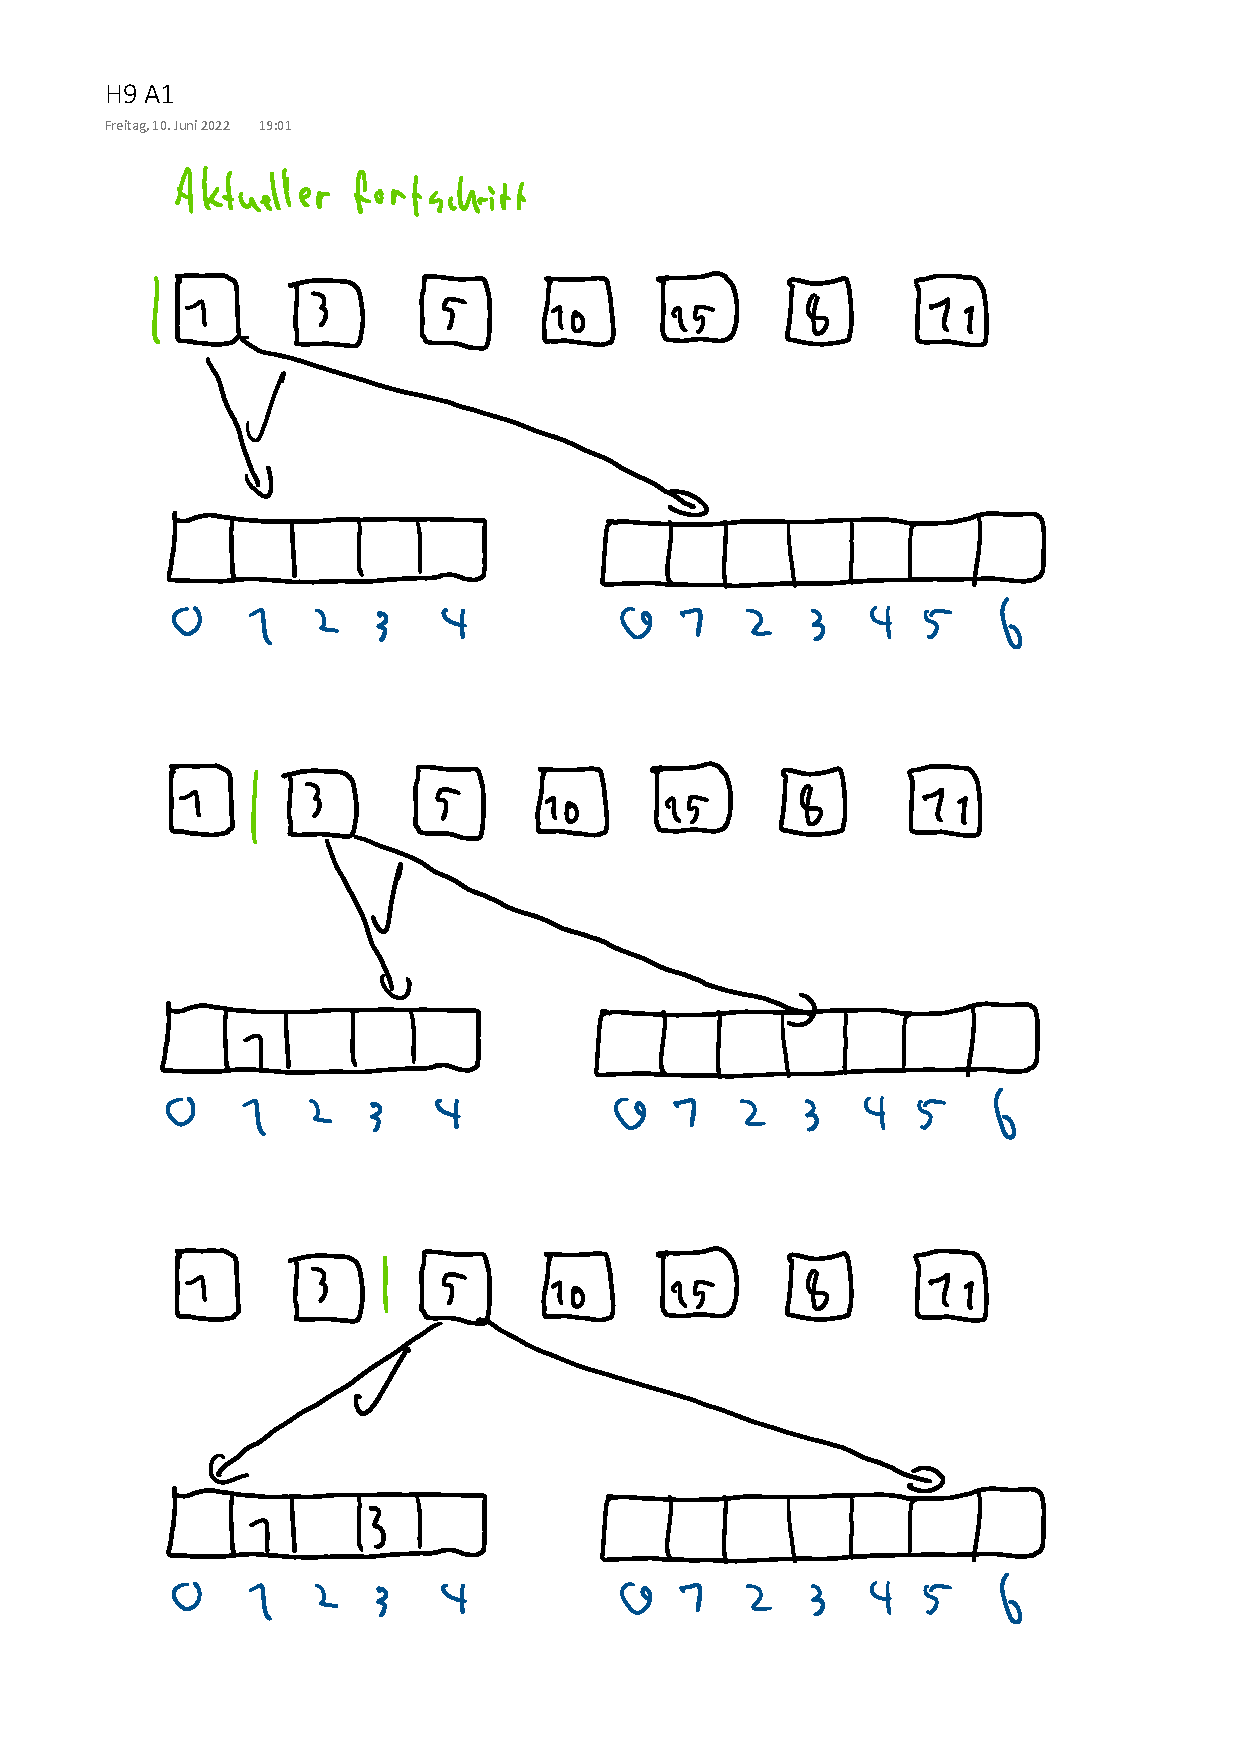
\includepdf[pages=-]{2022-06-10-Blatt-9-Aufgabe-1-1.pdf}
  \end{teilaufgabe}
\end{aufgabe}
\begin{aufgabe}
  Bekannt sind Hashtablellen mit der Backing-Struktur ``Liste''.

  Wir ersetzen die Backing-Struktur mit einem AVL-Baum.

  % \textbf{Insert(T,x):}
  % Falls key[x] noch nicht in Baum T[h(key[x])] vorhanden, füge x in Baum T[h(key[x])] ein.

  \begin{algorithm}[H]
    \caption{\textsc{Insert}($T, x$)}
    \begin{algorithmic}[1]
      \State \textbf{Insert-AVL(T[h(key[x])], x)}
    \end{algorithmic}
  \end{algorithm}

  % \textbf{Delete(T,x):}
  % Falls key[x] in Baum T[h(key[x])] vorhanden, entferne x aus Baum T[h(key[x])].

  \begin{algorithm}[H]
    \caption{\textsc{Delete}($T, x$)}
    \begin{algorithmic}[1]
      \State \textbf{Delete-AVL(T[h(key[x])], x)}
    \end{algorithmic}
  \end{algorithm}

  % \textbf{Search(T,x):}
  % Falls key[x] in Baum T[h(key[x])] vorhanden, liefere true, sonst false.

  \begin{algorithm}[H]
    \caption{\textsc{Search}($T, x$)}
    \begin{algorithmic}[1]
      \State \textbf{Search-AVL(T[h(key[x])], x)}
    \end{algorithmic}
  \end{algorithm}

  Die Korrektheit ist durch die funktional identische Semantik zu Hashtablellen mit Backing-Liste gegeben.

  Durch Ersetzung der Backing-Struktur der ``Liste'' mit einem AVL-Baum ersetzen wir die
  zuvor bekannten Operationen mit Worst-Case Laufzeiten $O(n)$ durch $O(log n)$.
\end{aufgabe}
\begin{aufgabe}
  \begin{teilaufgabe}
    Beweis durch vollständige Induktion über die Kreislänge$:=n$:

    Wir verwenden die Kreisnotation $(x_1,x_2,\cdots,x_n)$ für einen Kreis über einen Graphen $G$.


    \begin{tikzpicture}
      [nodePath/.style={circle,fill=yellow!40}]
      \node[nodePath] (n1) at (0,0) {$x_1$};
      \node[nodePath] (n2) at (1,1) {$x_2$};
      \node[nodePath] (nn) at (2,0) {$x_n$};

      \foreach  \from/\to in {n1/n2,nn/n1}
      \draw[->] (\from) -- (\to) node [midway, auto] () {};

      \foreach \from/\to in {n2/nn}
      % dotted line
      \draw[dashed, ->] (\from) -- (\to) node [midway, auto] () {};
    \end{tikzpicture}

    \textbf{I.A.:} $n=1$: trivial

    $n=2$:

    Wir betrachten die Möglichen Kreise $K_1=(x_1,x_2)$ $K_2=(x_1,x_1)$.

    $K_1$ ist ein einfacher Kreis.

    $K_2$ ist ein komplexer Kreis.

    $K_2$ kann in die einfachen Kreise $(x_1)$ und $(x_1)$ aufgeteilt werden.

    \rule{\textwidth}{0.5pt}

    Sei $n\in \mathbb{N}$.

    \textbf{I.V.:} Jeder komplexe Kreis mit bis zu $n-1$ Knoten kann in einfache Kreise aufgeteilt werden.

    \textbf{I.S.:} Sei $K_n=(x_1,x_2,\cdots,x_{i-1},x_i,\cdots,x_{j-1},x_j\cdots,x_n)$ ein komplexer Kreis.

    Existieren kein $1\leq i\neq j\leq n$: $x_i=x_j$ so ist der Kreis einfach.

    Also existieren $1\leq i\leq n$: $x_i=x_j$.

    Nun sind $K_a=(x_1,x_2,\cdots,x_{i-1},x_j,\cdots,x_n)$ und $K_b=(x_i,x_j,\cdots,x_{j-1})$ Kreise.

    Sind $K_a$ und $K_b$ einfach, so sind wir fertig.
    Sind sie komplex, so können wir sie nach \textbf{I.V.}
    in einfache Kreise $K_a=K_{a_1}+K_{a_2}+\cdots+K_{a_k}$,
    $K_b=K_{b_1}+K_{b_2}+\cdots+K_{b_l}$ aufteilen.

    Nun sind ist $K_{a_1},K_{a_2},\cdots,K_{a_k},K_{b_1},K_{b_2},\cdots,K_{b_l}$ eine Aufteilung von $K_n$ in einfache Kreise.

    \qed
  \end{teilaufgabe}
  \begin{teilaufgabe}
    ``$\implies$'':

    Sei $G$ ein Graph mit einem Eulerkreis
    $E=(x_1,x_2,\cdots,x_{i-1},x_i,x_{i+1},\cdots,x_n)$.

    Sei $x$ ein Knoten in $G$ und $i\in\{i_1,\cdots,i_k\}$ die $k$-Vorkommnisse von $x$ im Eulerkreis sind.

    Da nun $(x_{i-1},x_i)$ eine Eingangskante von $x$ ist, die maximal $1$-mal für ein $i$ vorkommt, ist $indeg(x)=k$.

    Da nun $(x_i,x_{i+1})$ eine Ausgangskante von $x$ ist, die maximal $1$-mal für ein $i$ vorkommt, ist $outdeg(x)=k$.

    Damit $indeg(x)=outdeg(x)$.


    \rule{\textwidth}{0.5pt}

    ``$\impliedby$'':

    Über Induktion über die Kantenanzahl $n$.

    \textbf{I.A.:} $n=1$: trivial, da $indeg\neq outdeg$ nicht vorkommt.

    \rule{\textwidth}{0.5pt}

    Sei $n\in\mathbb{N}$.

    \textbf{I.V.:} Jeder Graph mit $indeg(v)=outdeg(v)$ und maximal $n-1$ Kanten hat einen Eulerkreis.

    \textbf{I.S.:} Sei $G=(E,V)$ ein Graph mit $indeg(v)=outdeg(v)$ und $n$ Kanten.

    Bekannt ist, dass ein Kreis $K$ in $G$ existiert.

    Der Kreis $K$ geht über die Kantenmenge $E(K)$.

    Der Induzierte Teilgraph von $E\backslash E(K)$: $G_\text{ind}$ hat immernoch $indeg(v)=outdeg(v)$, da K im induzierte Teilgraph von $E(K)$ ein Eulerkreis ist.

    Nach \textbf{I.V.} hat $G_\text{ind}$ einen Eulerkreis, wir nennen ihn $K_\text{ind}$.

    Wir betrachten einen Knoten $v\in V(K)$.

    Wir stellen $K_\text{ind}$ als $K_\text{ind}=(v_1,v_2,\cdots,v_{i-1},v_i,v_{i+1},\cdots,v_k)$ dar,
    wobei $v=v_i$.

    Wir stellen $K$ als $K=(x_1,x_2,\cdots,x_{j-1},x_j,x_{j+1},\cdots,x_l)$ dar, wobei
    $v_i=v=x=x_j$.

    Nun ist $(v,v_{i+1},\cdots,v_k,v_1,\cdots,v_{i-1},v,x_{j+1},\cdots,x_l,x_1,\cdots,x_{j-1})$ ein Eulerkreis in $G$.
  \end{teilaufgabe}
\end{aufgabe}
\end{document}
